\section{Results and evaluation} \label{sec:results}

\subsection{Overview of datasets used for testing}
\label{sec:overview_of_datasets}

A couple of different datasets will be used for testing and evaluating the
implementation of the distance metrics and clustering algorithms presented in
section \ref{sec:methods}. These datasets will be briefly presented in this
section.

\begin{description}
  \item[\texttt{SILVA}] \hfill \\
    The dataset \texttt{SILVA\_119\_SSURef\_tax\_silva.fasta} has a size of
    around 2.3GB and contains $1,583,830$ RNA sequences.

  \item[\texttt{RDP}] \hfill \\
    The dataset \texttt{RDP\_Pro\_Full.sort.fna} has a size of around 3.5 GB
    and contains $3,019,928$ DNA sequences.
\end{description}

Various statistics about the datasets are shown in table \ref{tab:data_stats}.
The error ratio is the ratio between the number of non DNA/RNA bases, i.e. 'R',
'Y', 'K' etc., and the total number of characters in the sequences.

\begin{table}[H]
  \centering
  \begin{tabular}{c |  c | c | c | c | c}
    Dataset        & Avg. len. & Min. len. & Max. len. & Median len. & Error ratio \\
    \hline
    \texttt{SILVA} & 1,415.46  & 900       & 3,845     & 1,389       & 0.000156146 \\
    \texttt{RDP}   & 1,044.19  & 400       & 2,922     & 1,132       & 0.000798764 \\
  \end{tabular}
  \caption{Various information about the different datasets.}
  \label{tab:data_stats}
\end{table}


\subsection{Testing the distance metric on altered sequences}
\label{sec:altered_sequences}
%TODO: Misleading title?

Two different sets of highly similar sequences was constructed from a real
world sequence from \texttt{SILVA} and this was used in the evaluation of the
distance metric.

One sequence was chosen, 10 copies of this sequences were made and to each of
these copies, a few alterations were made. In the first set, a list of random
indices in the sequence were generated and in each of these indices in the
sequence, a substitution for a different, randomly chosen nucleotide was made.
This was done twice, for different degrees of alteration, and the number of
alterations was equal to respectively 1\% and 2\% of the length of the
sequence.

In the second set, the same number of alterations to individual nucleotides
were made, but in this case they were grouped into alterations of substrings of
length 5 (one such group being of length less than 5 if the number of
alterations was not a multiple of 5).

For illustration, figure \ref{fig:alterations} shows an original sequence in
the first line, the single edits alterated sequence in the second line and the
chunk alterated sequence in the third line.

\newcommand{\tc}[1]{\textcolor{red}{#1}}
\begin{figure}[H]
  \centering
  \texttt{AAAAAAAAAAAAAAAAAAAAAA} \\
  \texttt{AAAAA\tc{T}AA\tc{C}AAAA\tc{G}AAAA\tc{T}AAA} \\
  \texttt{AAA\tc{TC}AAAAAAAAAA\tc{GG}AAAAA}
  \caption{Two types of alterations to sequences: the original sequence in the
    first line, single edit alterations in the second line and chunks of edits
    in the third line.}
  \label{fig:alterations}
\end{figure}

The $k$-mer based distance metric, presented in section
\ref{sec:kmer_distance}, is expected to be more sensitive to a number of
individual changes than to the same number of changes made in chunks. This test
serves to confirm this expectation and to give an insight into the change in
$k$-mer distance when performing a controlled number of edits.

The similarities between the original sequence from \texttt{SILVA} and the 10
altered sequences, for the four different types of alterations, are shown in
table \ref{tab:altered_seqs_similarities}.

\begin{table}[H]
  \centering
  \begin{tabular}{c|c||c|c}
    \multicolumn{2}{c||}{single edits}  & \multicolumn{2}{c}{chunk edits} \\
    \hline\hline
    1\%   &   2\%                   &   1\%   &   2\% \\
    \hline
    0.944   & 0.889                     & 0.980     & 0.960 \\
    0.947   & 0.887                     & 0.979     & 0.960 \\
    0.944   & 0.893                     & 0.979     & 0.960 \\
    0.941   & 0.902                     & 0.979     & 0.961 \\
    0.944   & 0.894                     & 0.979     & 0.958 \\
    0.947   & 0.894                     & 0.979     & 0.958 \\
    0.941   & 0.895                     & 0.982     & 0.958 \\
    0.945   & 0.891                     & 0.979     & 0.961 \\
    0.945   & 0.889                     & 0.979     & 0.958 \\
    0.946   & 0.897                     & 0.981     & 0.958
  \end{tabular}
  \caption{Similarity measures, using $k=6$, for 1\% and 2\% single edits, respectively,
    and 1\% and 2\% chunk edits, respectively, to 10 copies of a single
    sequence.}
  \label{tab:altered_seqs_similarities}
\end{table}

As expected, the single edits result in a lower similarity that the
corresponding chunk edits. This is because five individual changes will affect
the count of up to $5 \cdot k$ $k$-mers, while five changes in sequence will
only affect up to $4+k$ $k$-mers.


\subsection{Comparing \textsc{K-Dist} with the Levenshtein distance metric}

This section compares the implementation of the \textsc{K-Dist} distance metric
(algorithm \ref{alg:K-Dist}) with the implementation of the bottom-up dynamic
programming (DP) algorithm (algorithm \ref{alg:levenshtein} in appendix
\ref{app:levenshtein_algorithm}) for the Levenshtein distance metric.

The data in table \ref{tab:levenshtein_vs_kdist_performance} shows how many
comparisons per second the implementation of Levenshtein and the implementation
of \textsc{K-Dist} can afford. This is shown for various values for the $k$
parameter.

\begin{table}[H] % TODO: we need to state which dataset and the lengths of seqs
  \centering
  \begin{tabular}{ c | c }
    Distance metric implementation  & Comparisons/second  \\
    \hline \hline
    Levenshtein (DP)                & $\sim 195$          \\ \hline
    \textsc{K-Dist}, $k=4$          & $\sim 91,500$       \\ \hline
    \textsc{K-Dist}, $k=5$          & $\sim 91,000$       \\ \hline
    \textsc{K-Dist}, $k=6$          & $\sim 89,000$       \\ \hline
    \textsc{K-Dist}, $k=7$          & $\sim 72,500$       \\ \hline
    \textsc{K-Dist}, $k=8$          & $\sim 46,000$       \\
  \end{tabular}
  \caption{Performance comparison between a dynamic programming (bottom up)
    Levenshtein implementation and \textsc{K-Dist} implementation with
    different values for parameter $k$.}
  \label{tab:levenshtein_vs_kdist_performance}
\end{table}

\begin{wrapfigure}{l}{0.55\textwidth}
  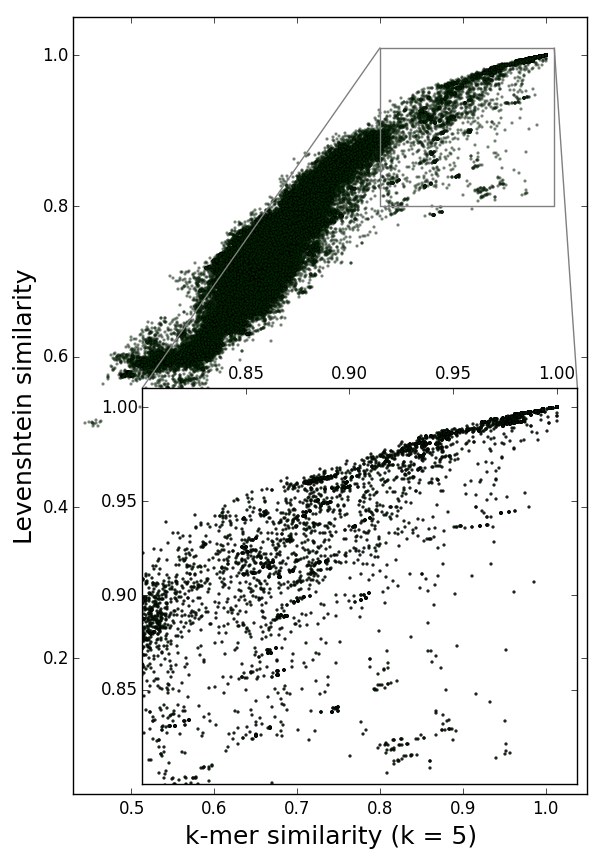
\includegraphics[width=0.55\textwidth]{graphics/Levenshtein_K-Dist_k5.png}
  \caption{Comparison of Levenshtein and \textsc{K-Dist} with $k=5$.}
\end{wrapfigure}

The \textsc{K-Dist} implementation with $k=4$ is more than 460 times faster
than the Levenshtein implementation, but becomes slower with increasing values
for $k$, with the \textsc{K-Dist} implementation being around 235 times faster
for $k=8$.

As mentioned in section \ref{sec:edit_distance}, the Levenshtein algorithm is
near quadratic in running time. As analyzed in section
\ref{sec:k-dist_analysis}, the \textsc{K-Dist} algorithm is

% TODO: insert running time of K-Dist

so it will always be faster that Levenshtein for long enough sequences and as
shown above in figure \ref{tab:levenshtein_vs_kdist_performance}, that is indeed
the case for the sequences this project is concerned with.

%As mentioned in section \ref{sec:edit_distance}, optimizing an implementation of
%distance metric to match the speed of \textsc{K-Dist} is unimaginable.


Despite its speed, it could be more sensible than \textsc{K-Dist}. Figure
\ref{fig:Levenshtein_vs_KDist} shows scatter plots of the Levenshtein distance
versus the distance \textsc{K-Dist} produces with different $k$'s. It
demonstrates how similar the distances are, and can be used as an indication
about the sensitivity of the \textsc{K-Dist} algorithm.


To evaluate the \textsc{K-Dist} algorithm, presented in section
\ref{sec:kmer_distance}, the Levenshtein distance was used as reference. Since
the Levenshtein distance does not produce values between 0 and 1, a similarity
ratio similar to the one used in \textsc{K-Dist} and expressed in equation
(\ref{eq:Manhattan_similarity}) was used. Specifically, the ratio between the
Levenshtein distance and the maximum possible distance subtracted from one. The
maximum possible Levenshtein distance is equal to the length of the longer
sequence.

\begin{figure}[H]
  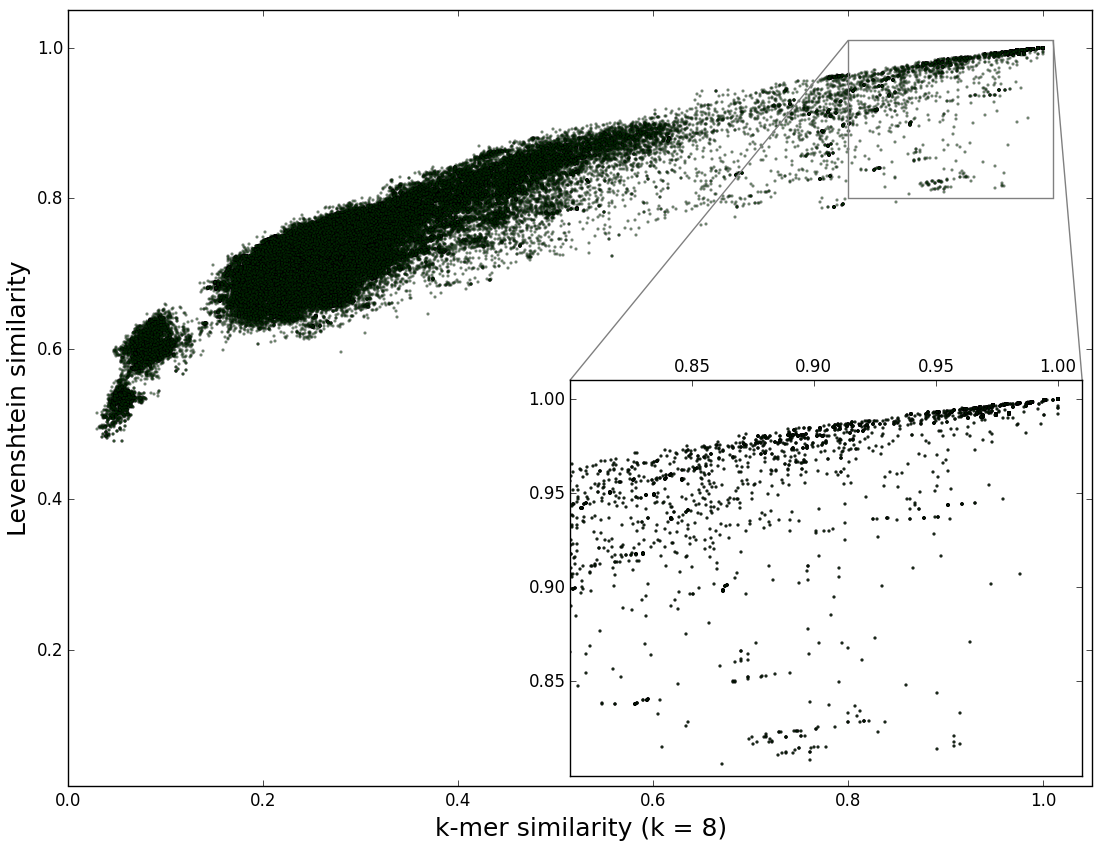
\includegraphics[width=1.0\textwidth]{graphics/Levenshtein_K-Dist_k8.png}
  \caption{Comparison of Levenshtein and \textsc{K-Dist} with $k=8$.}
  \label{fig:Levenshtein_vs_KDist}
\end{figure}


\subsection{Evaluating \textsc{K-Clust} on a synthetic dataset}
\label{sec:synth_dataset}

A synthetic dataset was constructed for evaluating the \textsc{K-Clust}
algorithm's ability to find the right clusters in a dataset with a clearly
correct, expected clustering output.

A set of 380 sequences with mutual similarities of at most 0.6 was extracted
from \texttt{SILVA}, using the \textsc{K-Dist} distance metric (algorithm
\ref{alg:K-Dist}) with parameter $k=5$. For each of these sequences, 999 copies
were made and chunks of changes were made to these as described above in
section \ref{sec:altered_sequences}, corresponding to 2\% of the characters of
each sequence. This yields a set of $380,000$ sequences with 380 expected
clusters, which each should contain sequences with similarities of
approximately $0.92$ since all sequences are changed and a 2\% change to a
sequence gives an average similarity from the original sequence of around
$0.96$, cf. section \ref{sec:altered_sequences}.

The sequences expected to be in the same cluster was given the same description
in the \texttt{FASTA} file, i.e. the same text string after ``>'', to make it
easy to evaluate the result from the clustering. Furthermore, the sequences
were placed in random order before running \texttt{klust} on the data.

The synthetic dataset was made fairly large, both in number of sequences and in
number of expected clusters, to be able to properly test the clustering
algorithm's ability to search for the correct centroid and not stop the search
prematurely which would result in a new cluster being created and a different
clustering result than the expected one.

As hoped, running \texttt{klust} on the constructed dataset, with parameters
$k=5$, $id=0.85$ and $max\_rejects=8$ gives a clustering output consisting of
380 clusters with 1000 sequences in each (including the centroid). The terminal
output from the program is shown in figure \ref{fig:synth_silva_output} in
appendix \ref{app:synth_dataset} and an excerpt from the clustering ouput file
created by the program is shown in figure \ref{fig:synth_silva_clustering} in
the same appendix. This shows that the sequences in each cluster have the same
description line, i.e. they were constructed to be similar and should indeed be
in the same cluster. The result was equally correct when clustering with a
threshold parameter of $0.89$, but the results start containing a few errors
when clustering with a threshold of $0.9$ or above. In the specific test, and
the specific, random order of the sequences, the clustering result yielded 386
clusters for $id=0.9$, average cluster size of $984.456$ and a minimum cluster
size of $33$.

% TODO: maybe add something like the following:
% This threshold is, however, close to the expected similarity of $0.92$ and
% since the clustering algorithm does not call \textsc{K-Dist} on every
% sequence/centroid pair, these errors can likely be contributed to
% \textsc{K-Clusts}'s choice of whether to call \textsc{K-Dist} or not, along
% with standard error.

This test provides some evidence that \textsc{K-Clust} is able to successfully
cluster a dataset of a fairly realistic size. Since the similarities are known
a priori and the cluster sequences are constructed to be of a similarity around
$0.92$ on $k=5$, this is not a test of the \textsc{K-Dist} distance metric.


\subsubsection{Multidimensional scaling of the synthetic dataset}
\label{sec:mds_synth}

\emph{Multidimensional scaling} (MDS) of the sequences in the synthetic data
set was used to visualize and further evaluate the clustering result from the
previous section (section \ref{sec:synth_dataset}). Multidimensional scaling
is used to visualize the distances between all the sequences in the synthetic
dataset in two dimensions, i.e. a scatter plot that tries to maintain the
relative distances between the sequences as well as possible.

The technique used for dimensionality reduction was \emph{t-distributed
Stochastic Neighbor Embedding} (t-SNE)~\cite{maaten}. This was done using
\texttt{Python} with \texttt{matplotlib} and \texttt{scikit-learn}. Sequences
expected to be in the same cluster were given the same color and thus the MDS
is expected to give a visualization of separate clusters of points of the same
color. Centroids were given a cirle marker and all other sequences were gives a
``+'' marker.

A subset of the synthetic set described in section \ref{sec:synth_dataset} was
used for the MDS, because the scatter plot easily becomes too densely populated
and because the computation is too expensive for $380,000$ sequences. A set of
400 sequences, consisting of 40 expected clusters with 10 sequences in each,
was used for the visualization shown in figure \ref{fig:mds_synth}.

\begin{figure}[H]
  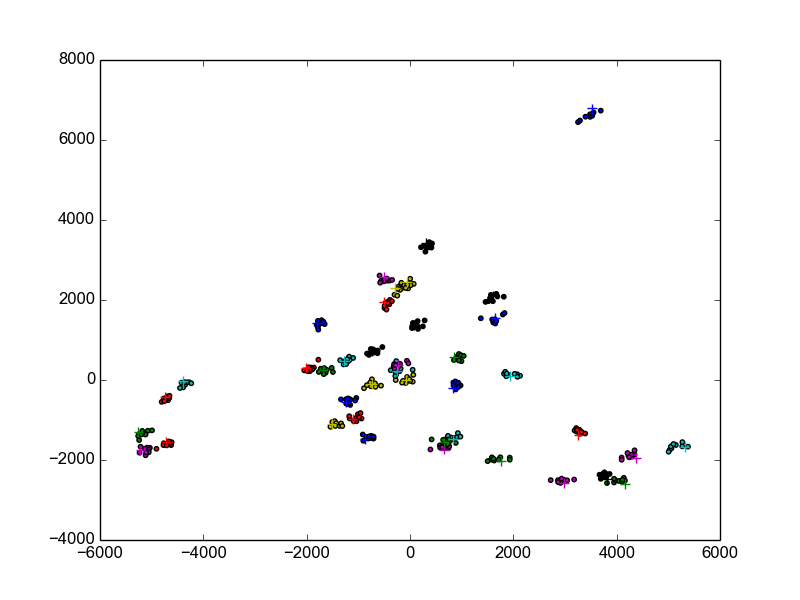
\includegraphics[width=\textwidth]{graphics/MDS_t-SNE_synth_silva_400.png}
  \caption{Multidimensional scaling using t-SNE of the 400 sequences and
    40 expected clusters from the synthetic dataset described in section
    \ref{sec:synth_dataset}. Centroids are marked with a cirle.}
  \label{fig:mds_synth}
\end{figure}

% TODO: discussion of the MDS figure


\subsection{Evaluating \textsc{K-Clust} on real data using MDS}

The \textsc{K-Clust} was also tested on real data, specifically the
\texttt{SILVA} dataset, using MDS to visualize the clustering result as
described in section \ref{sec:mds_synth}.

The clustering result from \texttt{klust} on \texttt{SILVA} consists of
clusters of very different sizes and a large number of singleton clusters, i.e.
clusters containing only the centroid sequence. This means that this data will
be harder to visualize nicely with MDS, since the clusters wont be as clearly
defined as with the synthetic dataset, but it should at least be possible to
identify the sequences of large clusters and observe whether they are indeed
close to each other in the MDS.

% TODO: insert MDS figures and discuss

\subsection{Evaluating \texttt{klust} on real data}

% TODO
% One example of this multidimensional scaling on the distance matrix for the
% first 500 sequences of \texttt{SILVA} is shown in figure \ref{fig:mds_tsne}.
% The centroids found using the clustering algorithm \textsc{K-Clust}, with
% similarity threshold 0.85, $max\_rejects$ 8 and $k$ 6, are pinpointed in the
% plot and labeled with the numbers of the sequences in the order they were read.

% \begin{figure}[h!]
%   \centering
%   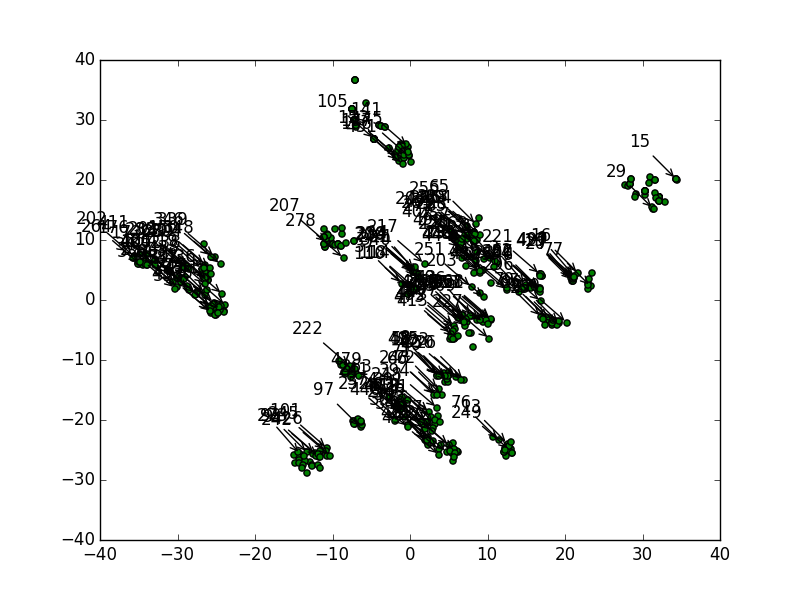
\includegraphics[width=\textwidth]{graphics/MDS_t-SNE_SILVA_500.png}
%   \caption{Multidimensional scaling with annotations on centroids.}
%   \label{fig:mds_tsne}
% \end{figure}

To test the performance and quality of the program, it was run on different
parameters and settings. The table in \ref{app:klust_data_parameters} shows
output data from running the first $100,000$ sequences from \texttt{SILVA}
with different parameters. Sorting by increasing length is on average
$21.65\%$ faster and never slower than not sorting. It is also on average
$42.63\%$ faster and never slower than sorting by decreasing length.
Furthermore, sorting by increasing length on average has $8.77\%$ fewer
clusters and never more clusters than not sorting. It has $25.07\%$ fewer
clusters on average and never more clusters than when sorting by decreasing
length. Generally higher $k$'s are also expected to produce more clusters,
since the comparison punishes mismatches more than lower $k$'s as discussed in
section \ref{sec:altered_sequences}.

The data shows that sorting by increasing length is always preferrable. The
higher $k$'s are also generally much slower and the comparisons are very
strict, i.e. the identity should be lower for the higher $k$. Section
\ref{sec:synth_dataset} and the multidimensional scaling plots in
\ref{fig:mds_synth} and \ref{fig:mds_silva_sort_incr} shows that $k=5$ is a good choice in terms of sensitivity.
Another interesting choice is $k=6$, since it does almost the same comparisons
per second (cf. figure \ref{tab:levenshtein_vs_kdist_performance}). These
results gives the incentive to study $k=5$ and $k=6$, when sorting by
increasing length, further.
%TODO: Why not k4?

In appendix \ref{app:performance_results_full_SILVA} is a table that shows
data from \texttt{klust} using either \textsc{K-Clust} or \textsc{Simple-Clust} and
\texttt{USEARCH}. The programs have been run with different parameters on the
entire \texttt{SILVA} dataset. Table
\ref{tab:full_silva_main_results} shows the most important results
found in appendix \ref{app:performance_results_full_SILVA} and appendix \ref{app:cluster_results_full_SILVA})


\begin{table}[H]
  \begin{adjustbox}{center}
  \begin{tabular}{c|c|c|c|cc|c}
  \multirow{2}{*}{}
  Clustering & Time & Throughput & Clusters & \multicolumn{2}{c}{Cluster sizes}& Max \\
  algorithm & (sec.) & (seqs./sec.) & & & & memory \\
  \hline \hline
  \multirow{3}{*}
  {}\textsc{Simple-Clust}, & & & & Max & - & \\
  $k=6, id=0.85, m=32,$    & 474.117 & 3340.59 & 1273293 & Avg. & 1.2439 & - \\
  no sort                  & & & & Min & 1 & \\
  \hline
  \multirow{3}{*}
  {}\textsc{K-Clust},  & & & & Max & 57885 & \\
  $k=5, id=0.85, m=8,$ & 1144.55 & 1383.81 & 98354 & Avg. & 16.1034 & 1013 MB \\
  incr. sort           & & & & Min & 1 & \\
  \hline
  \multirow{3}{*}
  {}\textsc{K-Clust},  & & & & Max & 71407 & \\
  $k=5, id=0.90, m=8,$ & 2578.88 & 614.155 & 159812 & Avg. & 9.91058 & 1021 MB\\
  incr. sort           & & & & Min & 1 & \\
  \hline
  \multirow{3}{*}
  {}\textsc{K-Clust},  & & & & Max & 79599 & \\
  $k=6, id=0.85, m=8,$ & 1812.02 & 874.066 & 127711 & Avg. & 12.4017 & 1012 MB\\
  incr. sort           & & & & Min & 1 & \\
  \hline
  \multirow{3}{*}
  {}\textsc{K-Clust},  & & & & Max & 49479 & \\
  $k=6, id=0.90, m=8,$ & 3450.59 & 459.003 & 191361 & Avg. & 8.27666 & 1039 MB\\
  incr. sort           & & & & Min & 1 & \\
  \hline
  \multirow{3}{*}
  {}\texttt{USEARCH},        & & & & Max & 83904 & \\
  $id=0.95,$ decr. sort      & 1719 & 920.3 & 117205 & Avg. & 13.5 & 1.1 GB \\
  \texttt{-cluster\_smallmem} & & & & Min & 1 & \\
  \end{tabular}
  \end{adjustbox}
  \caption{Performance and clusterings results of different clustering methods and different parameters on the entire \texttt{SILVA} dataset.}
  \label{tab:full_silva_main_results}
\end{table}
%TODO: explain table

\subsection{Comparing with UCLUST on real life data}
% Testing USEARCH 32-bit on real data
% Testing clustering algorithm with d2 distance and comparing performance to
% USEARCH.
Running \texttt{USEARCH} on the file
\texttt{SILVA\_119\_SSURef\_tax\_silva.fasta} after it is sorted with
parameters \texttt{-clust\_smallmem} and \texttt{-id 0.95} produces the
following output

\begin{figure}[H]
\begin{lstlisting}[style=output-style]
28:39 1.1Gb  100.0\% 117205 clusters, max size 83904, avg 13.5
      Seqs  1583830 (1.6M)
  Clusters  117205 (117.2k)
  Max size  83904 (83.9k)
  Avg size  13.5
  Min size  1
Singletons  67410 (67.4k), 4.3\% of seqs, 57.5\% of clusters
   Max mem  1.1Gb
      Time  28:41
Throughput  920.3 seqs/sec.
\end{lstlisting}
  \caption{Output from \texttt{USEARCH} clustering.}
  \label{fig:uclust_silva}
\end{figure}

Benchmarks from \textsc{K-Clust} can be seen in the previous section.
% Running our implementation of the same file but unsorted and with
% \texttt{id=0.9, k=6} og \texttt{max\_rejects=8} produces the following

% \begin{figure}[H]
% \begin{lstlisting}[style=output-style]
% Reading 1583830 sequences...
% Finished reading:
% Time: 24.8109 sec.
% Seqs/sec: 63836
% Clustering 1583830 sequences...
% 26.4602
% # of clusters: 1364006
% Finished clustering:
% Time: 187.355 sec.
% Throughput: 8453.63seqs/sec.
% \end{lstlisting}
% %TODO caption and label?
% \end{figure}

% Even though the \texttt{id}'s do not represent the same threshold due to it
% being two different distance metrics we do get a lot more clusters. Running
% it with similar \texttt{id}'s produces almost the same amount of clusters, so
% the problem lies in the way we choose our centroids we compare a query
% sequence with.

% Our implementation, however, is faster by a factor of $10$. This can be
% attributed to our choice of distance metric.

%TODO: This section is also chaos
%Possibly things to look into: confusion matrix, Rand index, normalized
%mutual information (article: Comparing Clusterings - An Overview).

%TODO: Yeah well, results not done - update tables with other algorithms etc.


\subsection{Evaluation of centroid search in \texttt{klust}}

